\documentclass[11pt,a4paper]{article}

% --- Paquetes Esenciales ---
\usepackage[T1]{fontenc}
\usepackage[utf8]{inputenc}
\usepackage[spanish,es-tabla]{babel}
\usepackage{amsmath}
\usepackage[margin=2.5cm]{geometry}
\usepackage{graphicx}
\usepackage{xcolor}
\usepackage{tcolorbox}
\tcbuselibrary{skins}
\usepackage{hyperref}
\usepackage{fancyhdr}
\usepackage{float}
\usepackage{booktabs}
\usepackage{titlesec}
\usepackage{enumitem}
\usepackage{tabularx}
\usepackage{caption}
\usepackage{subcaption}

% --- Colores Institucionales UNSAAC y CGB ---
\definecolor{unsaacblue}{RGB}{18, 52, 102}
\definecolor{cgbnavy}{RGB}{11, 37, 69}
\definecolor{cgbteal}{RGB}{19, 154, 140}
\definecolor{boxbg}{RGB}{248, 250, 252}
\definecolor{boxborder}{RGB}{203, 213, 225}

\hypersetup{
    colorlinks=true,
    linkcolor=unsaacblue,
    filecolor=unsaacblue,
    urlcolor=unsaacblue,
    citecolor=unsaacblue
}

% --- Encabezados y Pies de Página ---
\pagestyle{fancy}
\fancyhf{}
\fancyhead[L]{\small\textbf{UNSAAC} -- Ingeniería de Software I}
\fancyhead[R]{\small\textbf{Laboratorio 7}: Sprint Planning y ejecución inicial}
\fancyfoot[L]{\small\textbf{Grupo de Laboratorio} -- Semestre 2026-I}
\fancyfoot[R]{\thepage}
\renewcommand{\headrulewidth}{0.8pt}
\renewcommand{\footrulewidth}{0.4pt}

% --- Formato de Títulos ---
\titleformat{\section}{\Large\bfseries\color{unsaacblue}}{\thesection.}{0.5em}{}[\titlerule]
\titleformat{\subsection}{\large\bfseries\color{unsaacblue}}{\thesubsection.}{0.5em}{}
\titleformat{\subsubsection}{\normalsize\bfseries\color{unsaacblue}}{\thesubsubsection.}{0.5em}{}

% --- Cajas Destacadas ---
\newtcolorbox{infobox}[1]{
    colback=boxbg,
    colframe=unsaacblue,
    fonttitle=\bfseries\color{white},
    title={#1},
    arc=2mm,
    boxrule=1pt,
    left=10pt, right=10pt, top=8pt, bottom=8pt,
    enhanced
}

\begin{document}

% ==============================================================================
% CARÁTULA
% ==============================================================================
\begin{titlepage}
    \centering
    {\Large\textbf{UNIVERSIDAD NACIONAL DE SAN ANTONIO ABAD DEL CUSCO}}\\[0.25cm]
    {\large\textbf{FACULTAD DE INGENIERÍA ELÉCTRICA, ELECTRÓNICA, INFORMÁTICA Y MECÁNICA}}\\[0.15cm]
    {\large\textbf{ESCUELA PROFESIONAL DE INGENIERÍA INFORMÁTICA Y DE SISTEMAS}}\\[0.8cm]

    
\includegraphics[width=4.2cm]{capturas/logo_unsaac.png}\\[0.8cm]

    {\Large\textbf{INFORME DE LABORATORIO N° 7}}\\[0.3cm]
    {\LARGE\textbf{\color{unsaacblue}Sprint Planning y Ejecución Inicial}}\\[0.2cm]
    {\large\textbf{Proyecto: Centro de Capacitación e Inducción -- CGB Academy}}\\[0.15cm]
    {\normalsize Sprint 2: Onboarding (09/11/2026 -- 23/11/2026)}\\[0.8cm]

    \begin{infobox}{Datos de la Asignatura y Repositorios Oficiales}
        \textbf{Curso:} Ingeniería de Software I (IF614)\\
        \textbf{Docente:} Ing. Lisha Sabah Diaz Caceres\\
        \textbf{Semestre Académico:} 2026-I\\
        \textbf{Repositorio en GitHub:} \url{https://github.com/milith0kun/proyecto-ing-software}\\
        \textbf{Backlog en Jira Cloud:} \url{https://cgb-academy.atlassian.net} (Proyecto: \textbf{CGB})
    \end{infobox}

    \vspace{0.4cm}

    \textbf{\large Integrantes del Grupo de Trabajo:}\\[0.2cm]
    \begin{tabularx}{\textwidth}{c X c l}
        \toprule
        \textbf{N°} & \textbf{Apellidos y Nombres} & \textbf{Código} & \textbf{Rol en el Sprint 2} \\
        \midrule
        1 & Barazorda Cuellar, Hector & 145003 & Desarrollador \\
        2 & Carpio Hermoza, Alex & 164563 & Desarrollador \\
        3 & Quispe Mamani, Domingo de Guzman & 191978 & Desarrollador \\
        4 & Saire Bustamante, Edmil Jampier & 174449 & Product Owner y Scrum Master \\
        5 & Ticona Jancco, Ronaldo & 211816 & Desarrollador \\
        \bottomrule
    \end{tabularx}

    \vfill
    {\small Cusco, Perú -- Noviembre de 2026}
\end{titlepage}

\tableofcontents
\newpage

% ==============================================================================
\section{Objetivo del Laboratorio}

Planificar el segundo sprint del proyecto CGB Academy: definir su duración y objetivo, seleccionar las historias de usuario según la capacidad del equipo, descomponerlas en tareas, asignarlas y dejar evidencia del inicio del desarrollo (ramas en Git y primer avance con TDD). Los datos de Jira citados se leyeron el 09/11/2026 mediante la API del proyecto \textbf{CGB}.

% ==============================================================================
\section{Fundamento Teórico}

\begin{itemize}[leftmargin=1.5cm]
    \item \textbf{Scrum y Sprint Planning:} el equipo acuerda qué se entregará en el sprint (\textit{objetivo}), por qué es valioso y cómo se construirá. La selección parte de la capacidad real del equipo y no del deseo de entregar más (Schwaber y Sutherland, 2020).
    \item \textbf{Sprint Backlog:} conjunto de historias seleccionadas más el plan para entregarlas. En Jira se materializa como las historias asignadas al sprint con sus subtareas.
    \item \textbf{Definition of Done (DoD):} criterios comunes y verificables para considerar terminada una historia; en el proyecto están en \texttt{docs/definition-of-done.md}.
    \item \textbf{Estrategia de ramas:} \textit{GitHub Flow}. Una sola rama permanente (\texttt{main}), una rama \texttt{feature} corta por historia, Pull Request revisado por otra persona y \textit{Squash and merge}.
\end{itemize}

% ==============================================================================
\section{Herramientas Utilizadas}

\begin{itemize}[leftmargin=1.5cm]
    \item \textbf{Jira Software Cloud:} proyecto CGB, sprint 2 (id 2), historias y subtareas.
    \item \textbf{GitHub:} repositorio \texttt{milith0kun/proyecto-ing-software}, ramas y Pull Requests.
    \item \textbf{Node.js, \texttt{tsx} y Prisma 6.19:} pruebas automáticas y validación del esquema de datos.
\end{itemize}

% ==============================================================================
\section{Desarrollo de las Actividades}

\subsection{Parte 1: Definición del Sprint}

\begin{table}[H]
\centering
\begin{tabularx}{\textwidth}{l X}
\toprule
\textbf{Elemento} & \textbf{Definición} \\
\midrule
Sprint & Sprint 2: Onboarding (estado \textit{activo} en Jira) \\
Duración & 2 semanas: 09/11/2026 -- 23/11/2026 \\
Product Owner y Scrum Master & Edmil Jampier Saire Bustamante \\
Desarrolladores (4) & Alex Carpio, Domingo Quispe, Ronaldo Ticona y Héctor Barazorda \\
\bottomrule
\end{tabularx}
\caption{Datos del Sprint 2.}
\end{table}

\begin{infobox}{Objetivo del Sprint 2 (cargado en Jira)}
Permitir que el administrador defina áreas, puestos y rutas de onboarding y registre colaboradores; que cada colaborador active su cuenta, consulte \textit{Mi Onboarding} y registre su avance; y dejar configurado y disponible el microtest formativo.
\end{infobox}

\textbf{Alcance excluido:} constancias, insignias y certificados (fuera del MVP, ver CGB-51). El reporte de avance (CGB-71, HU-015) permanece en el Sprint 3.

\subsection{Parte 2: Selección de Historias y Capacidad}

\textbf{Cambio de alcance respecto al Laboratorio 5.} Las historias CGB-61 (HU-013) y CGB-66 (HU-014), con 10 SP, se adelantaron del Sprint 3 al Sprint 2. El sprint pasó de 22 a \textbf{32 SP}, y el Sprint 3 queda con CGB-71 (5 SP). Esta decisión de alcance requiere aprobación del Product Owner registrada en Jira.

\textbf{Capacidad.} En el Sprint 1 se entregaron 19 SP con 3 desarrolladores ($\approx 6{,}3$ SP por persona); con 4 desarrolladores la capacidad equivalente es $\approx 25$ SP. El Sprint 2 compromete 32 SP, es decir 8 SP por persona, un 28\,\% por encima de esa capacidad. Es un compromiso \textbf{ambicioso}: si el sprint se retrasa, las candidatas a salir son HU-014 (CGB-66) y HU-012 (CGB-56).

\begin{table}[H]
\centering
\small
\begin{tabularx}{\textwidth}{l X c l l}
\toprule
\textbf{Clave} & \textbf{Historia} & \textbf{SP} & \textbf{Responsable (Jira)} & \textbf{Depende de} \\
\midrule
CGB-31 & HU-007: Crear área y puestos de trabajo & 3 & Alex Carpio & -- \\
CGB-36 & HU-008: Crear y secuenciar ruta de onboarding & 5 & Domingo Quispe & CGB-31 \\
CGB-41 & HU-009: Registrar colaboradores y asignar rutas & 3 & Ronaldo Ticona & CGB-31, 36 \\
CGB-46 & HU-010: Activar cuenta mediante token & 3 & Domingo Quispe & CGB-41 \\
CGB-51 & HU-011: Consultar panel personal Mi Onboarding & 5 & Ronaldo Ticona & CGB-36, 46 \\
CGB-56 & HU-012: Completar capacitación y registrar avance & 3 & Héctor Barazorda & CGB-51 \\
CGB-61 & HU-013: Configurar microtest formativo & 5 & Alex Carpio & HU-003 \\
CGB-66 & HU-014: Realizar microtest formativo interactivo & 5 & Héctor Barazorda & CGB-61 \\
\midrule
 & \textbf{Total} & \textbf{32} & 8 SP por persona & \\
\bottomrule
\end{tabularx}
\caption{Sprint Backlog del Sprint 2 con los responsables vigentes en Jira.}
\end{table}

Antes del reparto, Jira concentraba 15 SP en Domingo, 11 en Alex, 6 en Ronaldo y ninguno en Héctor. Se reasignaron CGB-46, CGB-51, CGB-56 y CGB-66 junto con sus 16 subtareas para que cada integrante tenga una historia de 3 SP y una de 5 SP.

\begin{figure}[H]
    \centering
    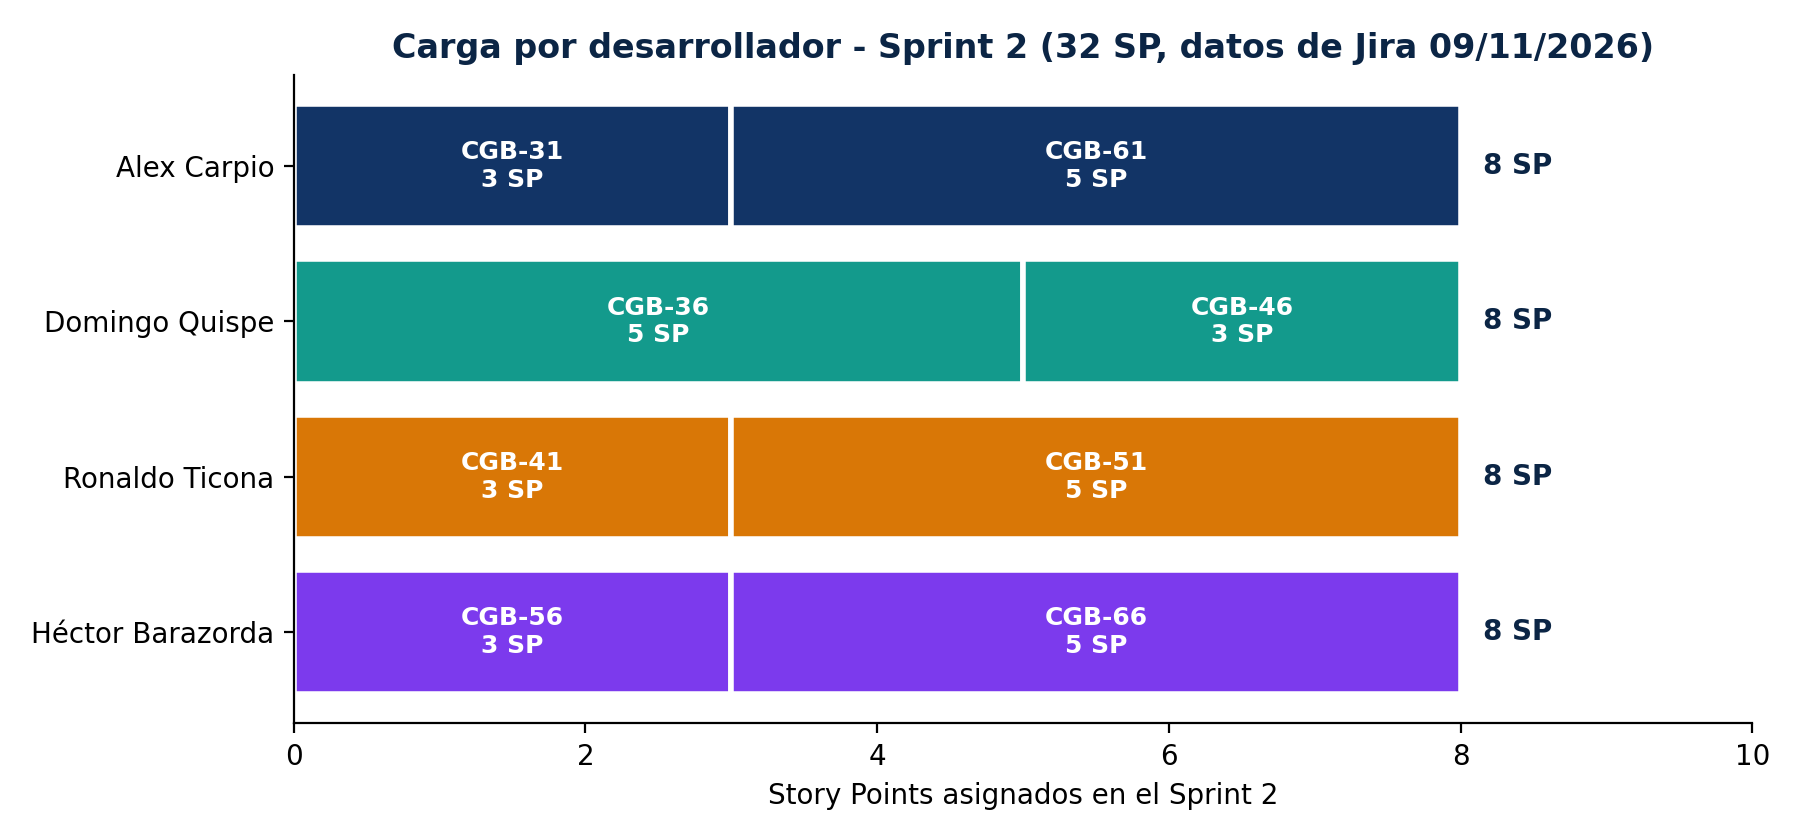
\includegraphics[width=0.95\textwidth]{capturas/grafico_carga_sprint2.png}
    \caption{Carga por desarrollador en el Sprint 2, generada con datos leídos de Jira el 09/11/2026.}
\end{figure}

\begin{figure}[H]
    \centering
    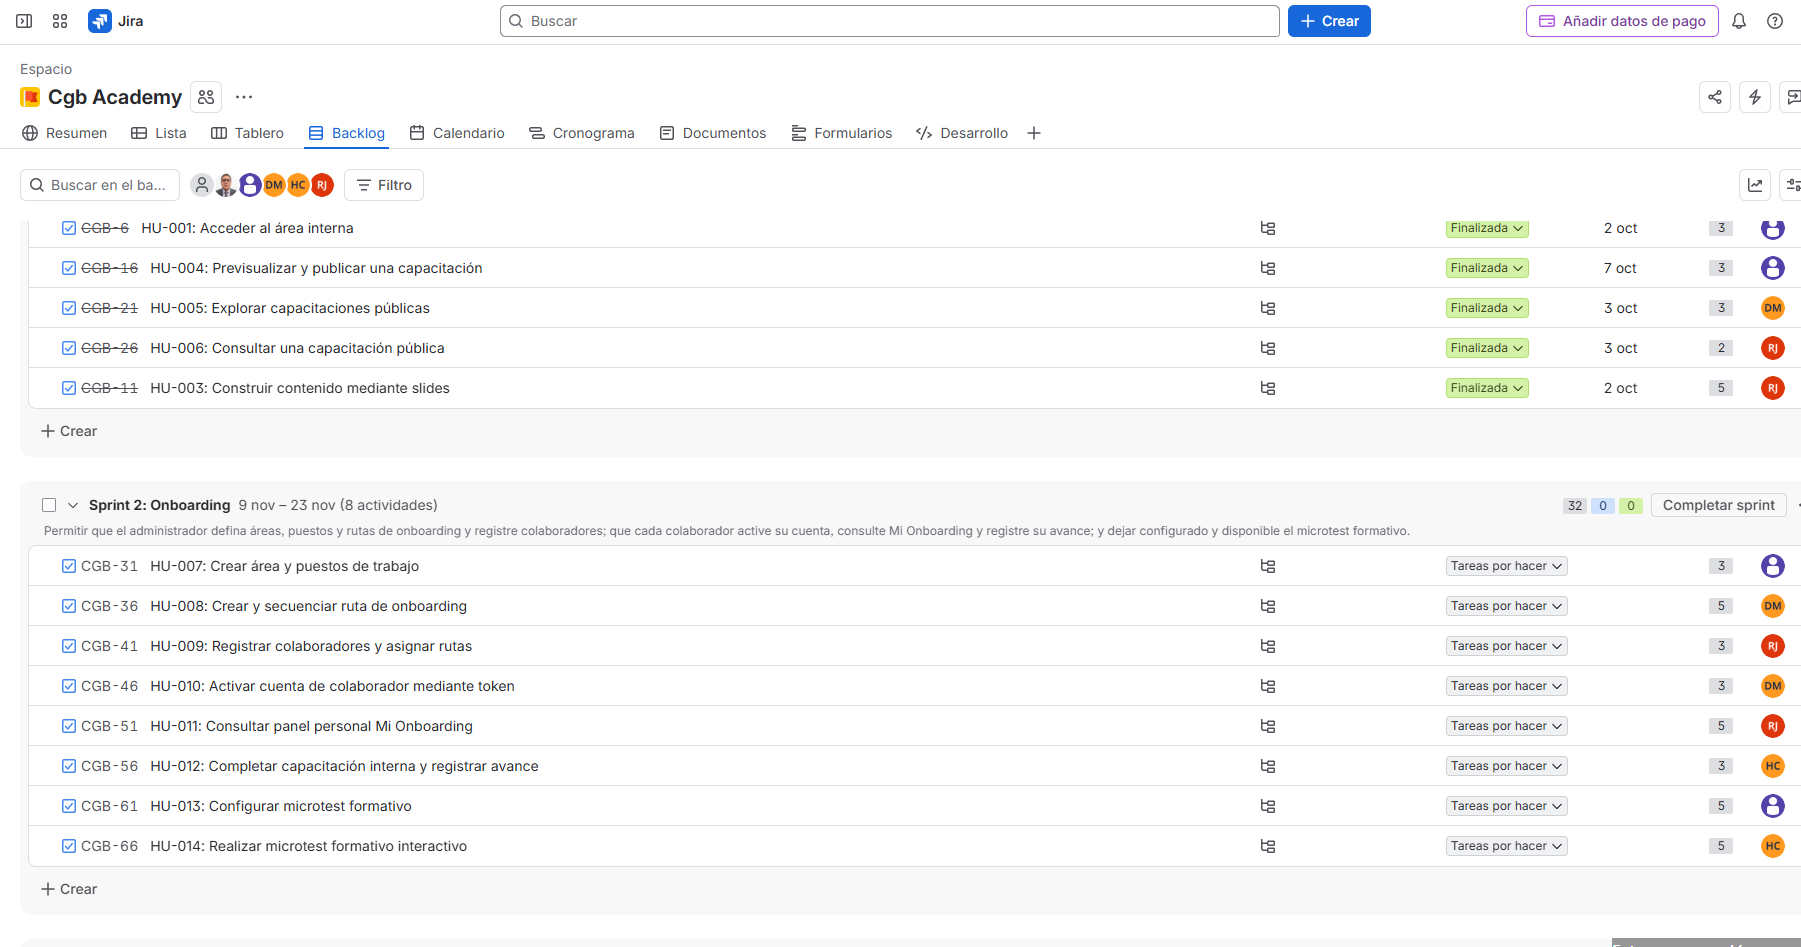
\includegraphics[width=0.98\textwidth]{capturas/captura_jira_backlog_sprint2.png}
    \caption{Backlog en Jira Cloud: Sprint 2 con su objetivo, 8 actividades, 32 SP y el responsable de cada historia (avatares). Captura del equipo.}
\end{figure}

\textbf{Riesgos identificados.}
\begin{enumerate}[label=\textbf{\arabic*.}]
    \item Carga de 32 SP por encima de la capacidad equivalente.
    \item Dependencias en cadena (CGB-31 $\rightarrow$ 36 $\rightarrow$ 41 $\rightarrow$ 46 $\rightarrow$ 51 $\rightarrow$ 56 y CGB-61 $\rightarrow$ 66). Mitigación: acordar el esquema Prisma el primer día.
    \item CGB-51 y CGB-56 llevan la etiqueta \texttt{evidence-pending}: aún no se entrevistó ni observó al colaborador y no se inventan hallazgos.
    \item Doble rol de Edmil (Product Owner y Scrum Master); las revisiones de código las hacen los desarrolladores entre sí.
    \item Privacidad (AG-C01): el avance de cada colaborador es dato personal y solo debe verlo el propio colaborador y el administrador.
\end{enumerate}

\textbf{Límite WIP.} Con cuatro desarrolladores, el límite de la columna \textit{Desarrollo} sube de 3 a \textbf{4} (una historia activa por desarrollador); \textit{Revisión} se mantiene en 2. El cambio está en \texttt{docs/FLUJO\_DE\_TRABAJO.md}, en el README y en el informe del proyecto.

\subsection{Parte 3: Descomposición en Tareas}

Cada historia tiene en Jira cuatro subtareas del ciclo TDD, asignadas al mismo responsable que la historia y todas en \textit{Tareas por hacer}:

\begin{table}[H]
\centering
\small
\begin{tabularx}{\textwidth}{l X}
\toprule
\textbf{Historia} & \textbf{Subtareas: T1 RED / T2 GREEN / T3 REFACTOR / T4 VALIDACIÓN} \\
\midrule
CGB-31 & CGB-32 / 33 / 34 / 35 \\
CGB-36 & CGB-37 / 38 / 39 / 40 \\
CGB-41 & CGB-42 / 43 / 44 / 45 \\
CGB-46 & CGB-47 / 48 / 49 / 50 \\
CGB-51 & CGB-52 / 53 / 54 / 55 \\
CGB-56 & CGB-57 / 58 / 59 / 60 \\
CGB-61 & CGB-62 / 63 / 64 / 65 \\
CGB-66 & CGB-67 / 68 / 69 / 70 \\
\bottomrule
\end{tabularx}
\caption{Subtareas existentes en Jira. Sus descripciones están vacías; el desglose siguiente es una propuesta para completarlas.}
\end{table}

\textbf{Contrato de datos del primer día} (extiende \texttt{prisma/schema.prisma}): \texttt{Area}, \texttt{PuestoTrabajo}, \texttt{RutaOnboarding} y \texttt{PasoRuta}, token de activación, \texttt{Avance} y las entidades del microtest.

\begin{table}[H]
\centering
\small
\begin{tabularx}{\textwidth}{l X}
\toprule
\textbf{Historia} & \textbf{Desglose técnico propuesto} \\
\midrule
CGB-31 & Modelos de área y puesto; validación con nombre único; API protegida por rol administrador; vista en acordeón. \\
CGB-36 & Modelos de ruta y pasos; solo capacitaciones internas publicadas; API de creación y reordenamiento. \\
CGB-41 & Alta de colaborador inactivo con puesto y ruta; correo duplicado; formulario de alta. \\
CGB-46 & Token de un solo uso con expiración; casos inválido, expirado y reutilizado; activación de cuenta. \\
CGB-51 & Consulta de la ruta del colaborador y porcentaje de avance; aislamiento entre usuarios. \\
CGB-56 & Modelo de avance; registro idempotente; integración con el visor de slides. \\
CGB-61 & Microtest con preguntas y opciones; validación de configuración; pantalla de administración. \\
CGB-66 & Intento, calificación y retroalimentación formativa; pantalla interactiva. \\
\bottomrule
\end{tabularx}
\caption{Desglose técnico propuesto por historia.}
\end{table}

\subsection{Parte 4: Inicio del Desarrollo}

\textbf{Estrategia de ramificación elegida: GitHub Flow.} Se descartó Git Flow (\texttt{develop}, \texttt{release}) porque el equipo es pequeño, los sprints duran dos semanas y existe una sola versión activa. La regla está en \texttt{docs/FLUJO\_DE\_TRABAJO.md}.

\begin{figure}[H]
    \centering
    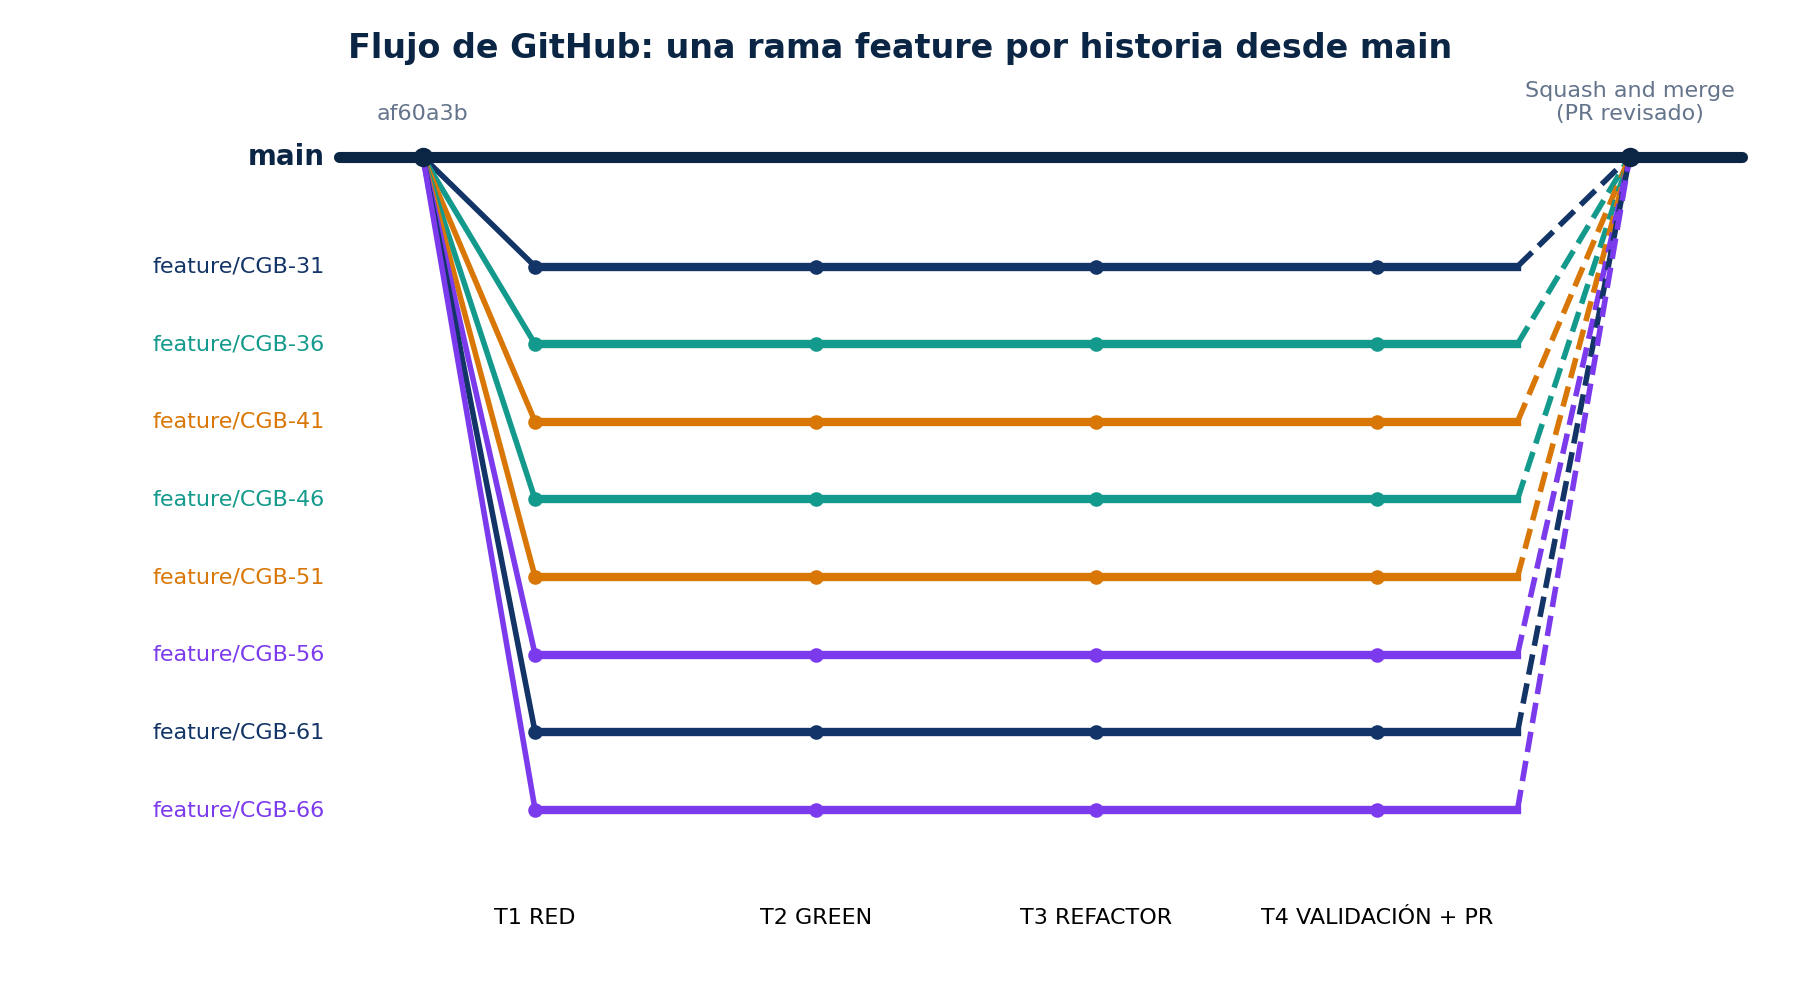
\includegraphics[width=0.95\textwidth]{capturas/diagrama_flujo_github.png}
    \caption{Ramas del Sprint 2 creadas desde \texttt{main} (commit af60a3b); cada una cierra con un Pull Request revisado.}
\end{figure}

\textbf{Ramas creadas y publicadas en GitHub} (formato \texttt{tipo/clave-jira-resumen}):

\begin{table}[H]
\centering
\small
\begin{tabularx}{\textwidth}{X l l}
\toprule
\textbf{Rama} & \textbf{Historia} & \textbf{Responsable} \\
\midrule
\texttt{feature/CGB-31-areas-y-puestos} & CGB-31 & Alex Carpio \\
\texttt{feature/CGB-36-ruta-onboarding} & CGB-36 & Domingo Quispe \\
\texttt{feature/CGB-41-registrar-colaboradores} & CGB-41 & Ronaldo Ticona \\
\texttt{feature/CGB-46-activar-cuenta-token} & CGB-46 & Domingo Quispe \\
\texttt{feature/CGB-51-mi-onboarding} & CGB-51 & Ronaldo Ticona \\
\texttt{feature/CGB-56-completar-capacitacion} & CGB-56 & Héctor Barazorda \\
\texttt{feature/CGB-61-configurar-microtest} & CGB-61 & Alex Carpio \\
\texttt{feature/CGB-66-realizar-microtest} & CGB-66 & Héctor Barazorda \\
\bottomrule
\end{tabularx}
\caption{Ramas del Sprint 2. Todas parten de \texttt{origin/main}; solo CGB-31 tiene ya un commit propio.}
\end{table}

\begin{figure}[H]
    \centering
    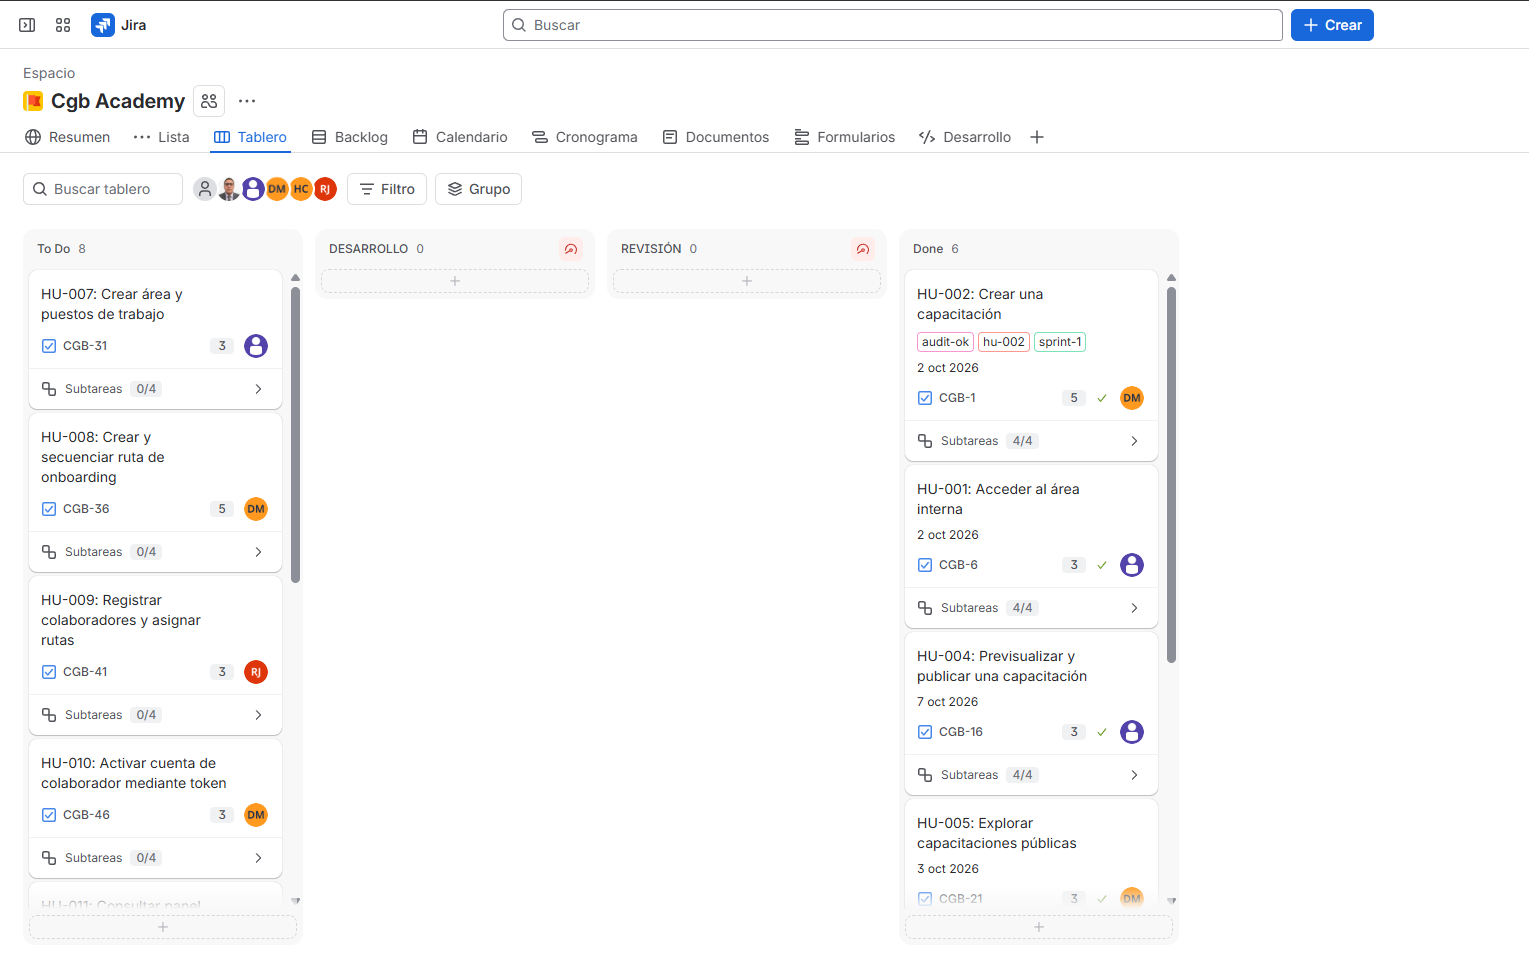
\includegraphics[width=0.95\textwidth]{capturas/captura_jira_tablero_sprint2.png}
    \caption{Tablero en Jira Cloud al inicio del Sprint 2: 8 historias en \textit{To Do} con 0/4 subtareas, columnas \textit{Desarrollo} y \textit{Revisión} vacías y las historias del Sprint 1 en \textit{Done}. Captura del equipo.}
\end{figure}

\textbf{Estado en Jira.} Responsables, objetivo del sprint y subtareas están cargados; se creó la tarea CGB-78 para la alineación documental; CGB-76 y CGB-77 se asignaron a Edmil; se enlazaron en Jira los Pull Requests y commits de las historias ya integradas (CGB-1, 6, 11, 16 y 21). Como muestra el tablero, todavía no se movió ninguna historia a \textit{En desarrollo} (0 en Desarrollo y 0 en Revisión).

% ==============================================================================
\section{Entregables}

\begin{table}[H]
\centering
\small
\begin{tabularx}{\textwidth}{X l}
\toprule
\textbf{Entregable} & \textbf{Estado} \\
\midrule
Sprint Backlog definido (8 historias, 32 SP, objetivo cargado en Jira) & Cumplido \\
Tareas asignadas (historias y 32 subtareas con responsable) & Cumplido \\
Ramas Git creadas y publicadas (8) & Cumplido \\
Primer commit de desarrollo (CGB-31) & Cumplido \\
Historias movidas a \textit{En desarrollo} en Jira & Pendiente \\
Límite WIP de 4 configurado en el tablero de Jira & Pendiente \\
Capturas del backlog y del tablero del Sprint 2 con el reparto actual & Cumplido \\
Captura de las ramas en GitHub y del commit de CGB-31 & Pendiente \\
Aprobación y fusión del PR \#7 (documentos de flujo, DoD y configuración) & Pendiente de revisión \\
\bottomrule
\end{tabularx}
\caption{Estado de los entregables del laboratorio.}
\end{table}

% ==============================================================================
\section{Trabajo Extra: Avance de Implementación (CGB-31 / HU-007)}

Se inició la implementación de la primera historia de la cadena de dependencias en \texttt{feature/CGB-31-areas-y-puestos}, commit \texttt{42eb4a4}, siguiendo TDD:

\begin{enumerate}[label=\textbf{\arabic*.}]
    \item \textbf{RED (T1):} \texttt{tests/organizacion.test.mjs} con 7 pruebas que cubren CA-01 a CA-04 (alta de área, puestos vinculados al área, duplicados y jerarquía con conteo de colaboradores). Falló porque el módulo aún no existía.
    \item \textbf{GREEN (núcleo de T2):} \texttt{src/lib/organizacion.ts} con validación, detección de duplicados sin distinguir mayúsculas ni tildes y armado de la jerarquía; y los modelos \texttt{Area} y \texttt{PuestoTrabajo} en \texttt{prisma/schema.prisma}.
\end{enumerate}

\textbf{Comprobaciones ejecutadas:} \texttt{npx tsx --test tests/organizacion.test.mjs} $\rightarrow$ 8 de 8 pruebas aprobadas; \texttt{prisma validate} (Prisma 6.19.3) $\rightarrow$ esquema válido.


% ==============================================================================
\section{Evidencia del Producto: Sprint 1 y Sprint 2}

Las capturas siguientes se tomaron el 09/11/2026 ejecutando la aplicación en un servidor local (\texttt{next dev}, puerto 3100) conectada a la base de datos del proyecto.

\subsection{Sprint 1: Capacitación y Acceso (historias finalizadas)}

\begin{figure}[H]
    \centering
    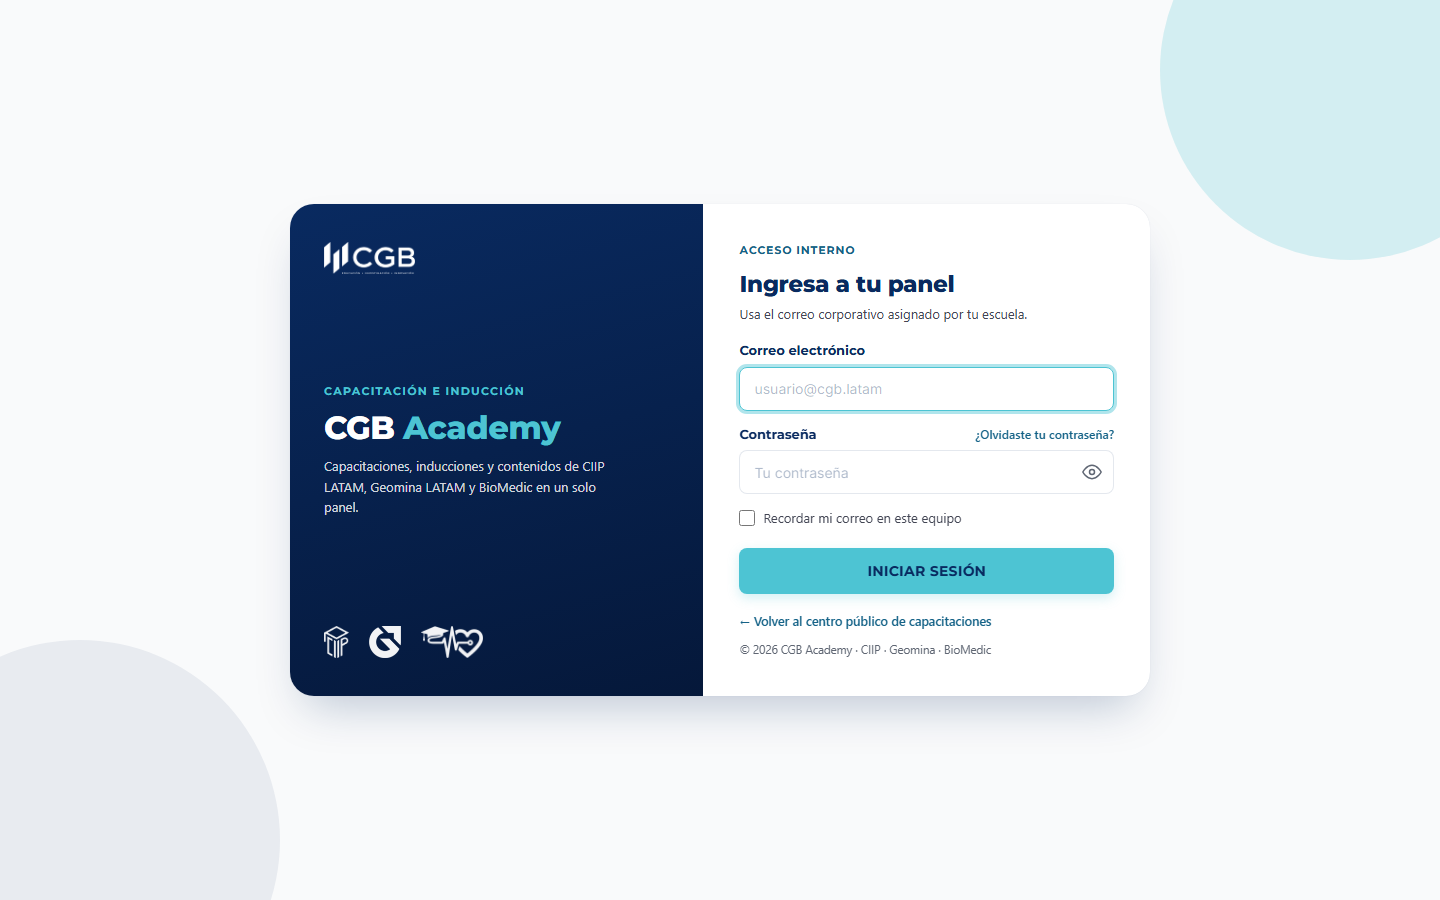
\includegraphics[width=0.85\textwidth]{capturas/captura_app_login.png}
    \caption{HU-001 (CGB-6): acceso interno con correo corporativo, contraseña y enlace de regreso al catálogo público.}
\end{figure}

\begin{figure}[H]
    \centering
    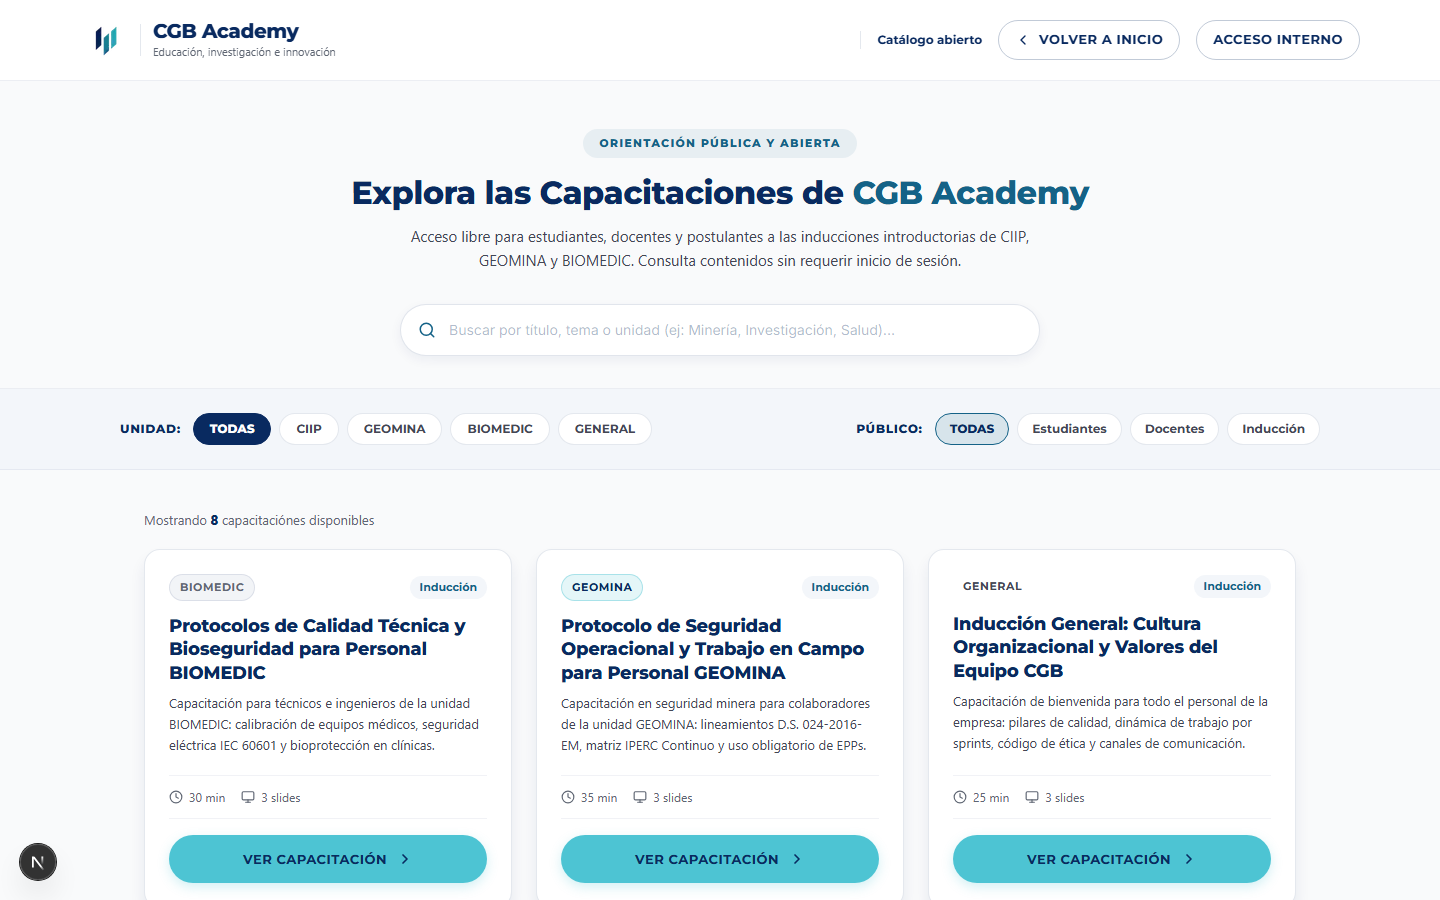
\includegraphics[width=0.85\textwidth]{capturas/captura_app_catalogo.png}
    \caption{HU-005 (CGB-21): catálogo público de capacitaciones con búsqueda y filtros por unidad y público (8 capacitaciones publicadas).}
\end{figure}

\begin{figure}[H]
    \centering
    
\includegraphics[width=0.85\textwidth]{capturas/captura_app_capacitacion.png}
    \caption{HU-006 (CGB-26): consulta de una capacitación pública con diapositivas y barra de progreso (``Diapositiva 1 de 3'').}
\end{figure}

\begin{infobox}{Alcance de las capturas}
Los paneles de administrador y de colaborador (HU-001, HU-002, HU-003 y HU-004) requieren iniciar sesión; las cuentas de prueba del script \texttt{prisma/seed.mjs} no existen en la base conectada, por lo que esas pantallas no se capturaron y no se ejecutó el seed para no escribir en la base compartida. El \textbf{registro de colaboradores} (HU-009, CGB-41) pertenece al Sprint 2 y aún no está implementado, por lo que no hay pantalla que capturar.
\end{infobox}

\subsection{Sprint 2: Onboarding (avance inicial)}

El Sprint 2 está en sus primeros días: todas las historias están en \textit{To Do} y todavía no hay pantallas nuevas. La evidencia disponible es la ejecución de las pruebas de CGB-31 en verde (sección anterior):

\begin{figure}[H]
    \centering
    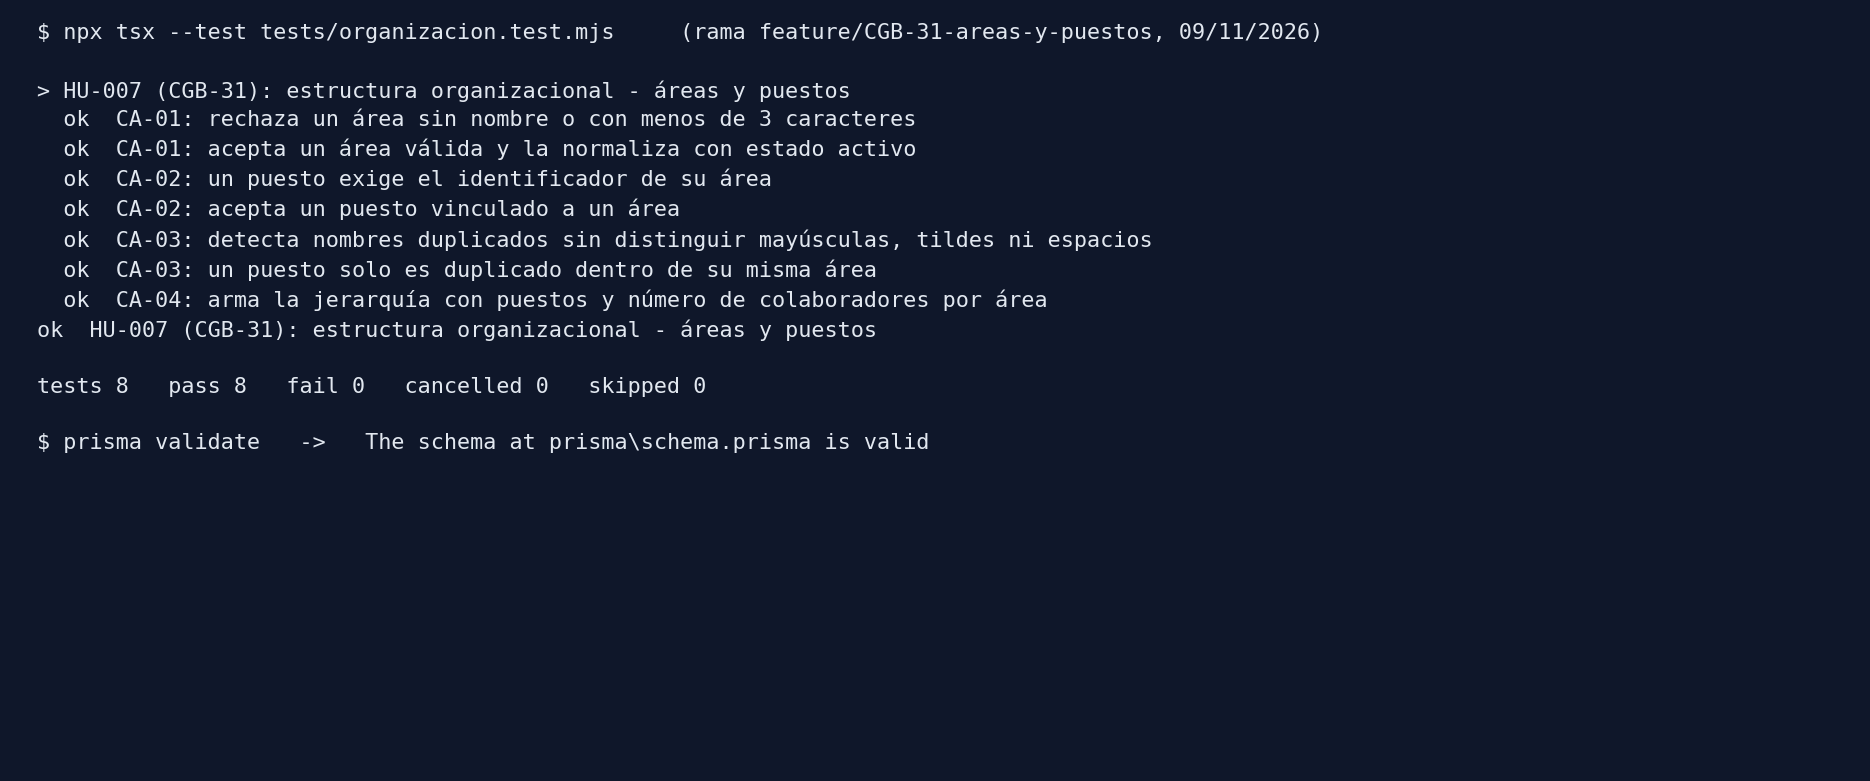
\includegraphics[width=0.95\textwidth]{capturas/captura_pruebas_cgb31.png}
    \caption{Salida de las pruebas de HU-007 (CGB-31) y validación del esquema Prisma en la rama \texttt{feature/CGB-31-areas-y-puestos}.}
\end{figure}

% ==============================================================================
\section{Conclusiones}

\begin{enumerate}[label=\textbf{\arabic*.}]
    \item La capacidad del equipo debe medirse con la velocidad real: al sumar un cuarto desarrollador y adelantar dos historias, el sprint pasó a 32 SP, por encima de los $\approx 25$ SP que sugiere el Sprint 1. Se dejó acordado qué historias salen primero si hay retraso.
    \item Repartir la carga explícitamente (8 SP por persona) evitó que un integrante concentrara 15 SP mientras otro no tenía trabajo, y se reflejó en Jira para que el tablero sea la fuente de verdad.
    \item Una sola rama permanente con ramas cortas por historia simplifica la integración para un equipo de cuatro personas, siempre que cada Pull Request lo revise alguien distinto del autor.
    \item El laboratorio queda con pendientes que dependen de personas, no del documento: la aprobación del PR \#7, el movimiento de historias a \textit{En desarrollo} y las capturas de GitHub.
\end{enumerate}

% ==============================================================================
\section{Referencias Bibliográficas}

\begin{itemize}[leftmargin=1.5cm]
    \item Schwaber, K. y Sutherland, J. (2020). \textit{The Scrum Guide}. \url{https://scrumguides.org/scrum-guide.html}
    \item GitHub Docs. \textit{GitHub flow}. \url{https://docs.github.com/}
    \item Conventional Commits 1.0.0. \url{https://www.conventionalcommits.org/en/v1.0.0/}
    \item Cohn, M. (2005). \textit{Agile Estimating and Planning}. Upper Saddle River, NJ: Prentice Hall PTR.
\end{itemize}

\end{document}
